\section{数据集与测试指标}

\subsection{语义分割评价指标}
\par 为评估系统性能,需要选择合适的评价指标,以量化系统在二维图像和三维点云模型语义分割中的准确性。以下是语义分割常用的评价指标。

\paragraph{像素精度(Pixel Accuracy,PA)}
\par 像素精度用于衡量语义分割图像中正确分类的像素数量与总像素数量之间的比例,是最基本的准确性度量指标,计算公式为
\begin{equation}
	PA=\frac{\sum_{i=1}^{k}p_{ii}}{\sum_{i=1}^{k}\sum_{j=1}^{k}p_{ij}}
	\label{pa}
\end{equation}

\par 其中,像素 $\text{p}_\text{ij}$ 表示将类别i预测为类别j。
像素精度的取值范围为 0 到 1,值越大表示语义分割结果越准确。但是,像素精度无法高效地反映类别不平衡的问题。

\begin{figure}[htb]
	\centering
	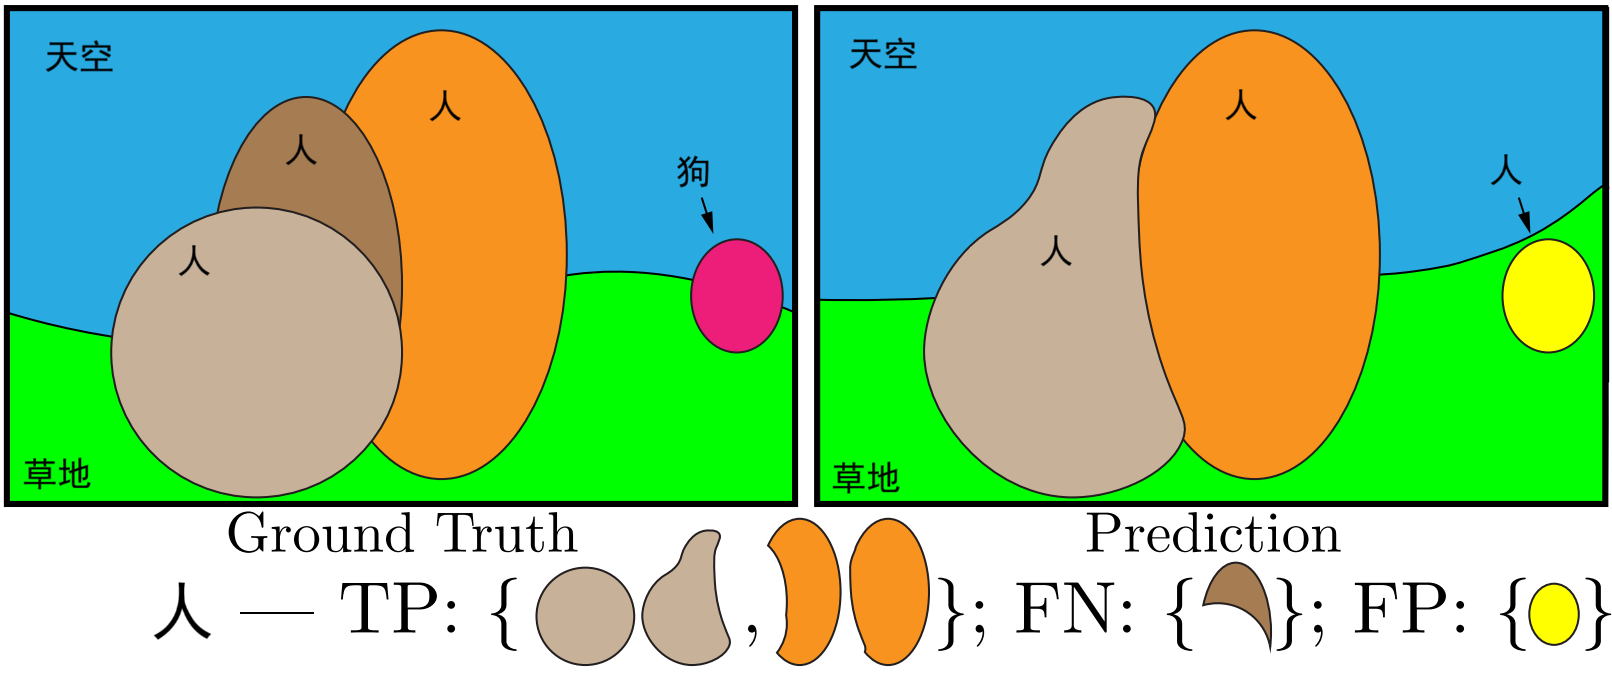
\includegraphics[width=0.9\textwidth]{figures/panoptic_seg_result.png}
	\caption{全景分割真实结果与预测结果的对比}
	\label{fig:panopticsegmentation_compare}
	\note{注:相同颜色的片段对表示交并比大于0.5则被匹配。图中展示了“person”类别的片段如何被分为 TP,FN 以及 FP。}
\end{figure}

\paragraph{平均交并比(Mean Intersection over Union,mIoU)}

\par mIoU是一个常用的衡量语义分割性能的指标。对于每一个类别,可以计算一个IoU值,然后将所有类别的IoU值取平均,得到mIoU。
每一个类别的IoU值是通过预测的类别区域(预测为该类别的像素点的集合)和真实的类别区域(真实标注为该类别的像素点的集合)的交集与并集的比值计算得出。mIoU的计算公式为
\begin{equation}
	mIoU = \frac{1}{C} \sum_{i=1}^{C}IoU_i = \frac{1}{C} \sum_{i=1}^{C}\frac{TP_i}{TP_i + FP_i + FN_i}
	\label{miou}
\end{equation}

\par 其中,C 是类别的总数,$\text{IoU}_\text{i}$ 是第i类的IoU值,$\text{TP}_\text{i}$ 是第i类的真阳性(True Positive)样本数量,$\text{FP}_\text{i}$ 是第i类的假阳性(FP)样本数量,$\text{FN}_\text{i}$ 是第i类的假阴性(False Negative)样本数量,
如图\ref{fig:panopticsegmentation_compare}\cite{panopticsegmentation}所示。

\par mIoU的取值范围为0到1,值越大表示语义分割性能越好。

\paragraph{频权交并比(Frequency Weighted Intersection over Union,FWIoU)}
\par FWIoU是对mIoU的一种变体,它考虑了类别的频率权重。对于频率较高的类别,其IoU值对总体性能的影响更大,可以解决类别不平衡的问题。计算公式为
\begin{equation}
	FWIoU = \sum_{i=1}^{C} \frac{p_i}{P} IoU_i = \sum_{i=1}^{C} \frac{p_i}{P} \frac{TP_i}{TP_i + FP_i + FN_i}
	\label{fwiou}
\end{equation}

\par 其中,C 是类别的总数,$\text{p}_\text{i}$ 是第i类的像素数,P是全部像素数。FWIoU值越高表示语义分割性能越好。

\paragraph{$\text{F}_\text{1}$ 分数($\text{F}_\text{1}$ Score)}
\par $\text{F}_\text{1}$分数综合考虑了预测精确率和召回率,适用于二分类问题,计算公式为
\begin{equation}
	F_{1} = \frac{2}{\frac{1}{Precision} + \frac{1}{Recall}} = \frac{2TP}{2TP+FP+FN}
	\label{f1score}
\end{equation}

\par 其中,Precision 是预测正样本中真正属于正类的比例,Recall 是实际正样本中被正确预测为正类的比例。$\text{F}_\text{1}$分数的范围是0到1,值越大表示语义分割性能越好。

% \paragraph{分割质量}
% \par SQ 是衡量预测分割准确性的指标。它通过计算预测分割与真实分割之间的 IoU 值来衡量准确性。SQ 的计算公式为

% \begin{equation}
% 	SQ=\frac{\sum_{(p,g) \in TP}IoU(p,g)}{|TP|}
% 	\label{sq}
% \end{equation}

% \par 其中,TP(True Positive)表示被判定为正例的正例,IoU 表示预测分割与真实分割之间的交并比。

% \paragraph{识别质量}
% \par RQ 是衡量类别识别准确性的指标。它通过计算预测类别与真实类别之间的 F1 分数来衡量准确性。RQ 的计算公式为

% \begin{equation}
% 	RQ=\frac{|TP|}{|TP|+\frac{1}{2}|FP|+\frac{1}{2}|FN|}
% 	\label{rq}
% \end{equation}

% \par 其中,FP(False Positive)表示被判定为正例的反例,FN(False Negative)表示被判定为反例的正例,如图\ref{fig:panopticsegmentation_compare}\cite{panopticsegmentation}所示。

% \begin{figure}[htb]
% 	\centering
% 	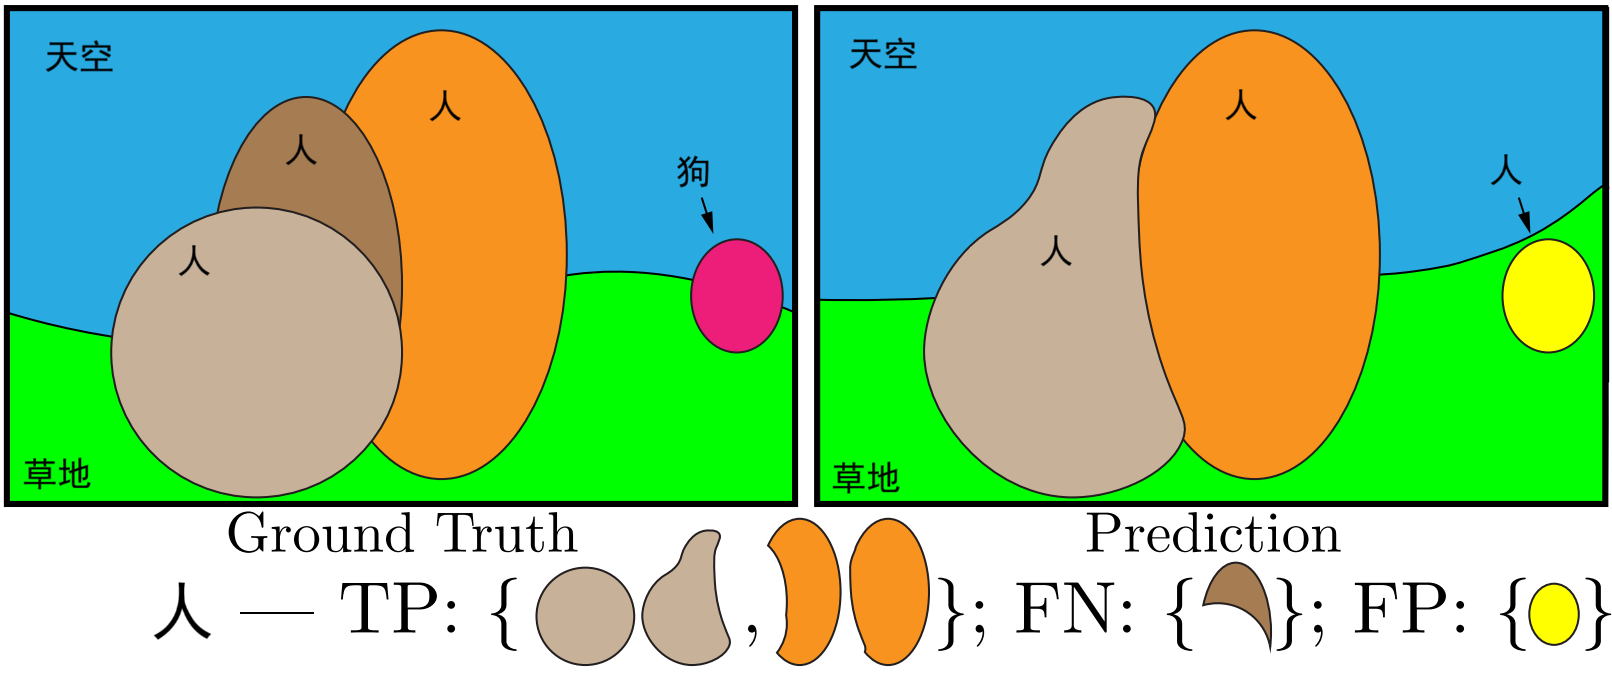
\includegraphics[width=0.9\textwidth]{figures/panoptic_seg_result.png}
% 	\caption{全景分割真实结果与预测结果的对比}
% 	\label{fig:panopticsegmentation_compare}
% 	\note{注:相同颜色的片段对表示交并比大于0.5则被匹配。图中展示了“person”类别的片段如何被分为 TP,FN 以及 FP。}
% \end{figure}

% \paragraph{全景分割质量}

% \par PQ 是衡量全景分割性能的主要指标,通过结合 SQ 和 RQ 计算得出。PQ 的计算公式为

% \begin{equation}
% 	PQ=SQ \times RQ=\frac{\sum_{(p,g) \in TP}IoU(p,g)}{|TP|+\frac{1}{2}|FP|+\frac{1}{2}|FN|}
% 	\label{pq}
% \end{equation}

% \par PQ的取值范围为0到1,值越大表示性能越好。

% \par 除了上述主要的评价指标,还有一些辅助指标可以帮助更全面地评估全景分割模型的性能:

% \paragraph{平均交并比(Mean Intersection Over Union,mIoU)}

% \par mIoU是一个常用的衡量语义分割性能的指标。对于每一个类别,可以计算一个IoU值,然后将所有类别的IoU值取平均,得到mIoU。
% 每一个类别的IoU值是通过预测的类别区域(预测为该类别的像素点的集合)和真实的类别区域(真实标注为该类别的像素点的集合)的交集与并集的比值计算得出。mIoU的计算公式为:

% \begin{equation}
% 	mIoU = \frac{1}{C} \sum_{i=1}^{C}\frac{|TP_i|}{|TP_i|+|FP_i|+|FN_i|}
% 	\label{miou}
% \end{equation}

% \par 其中,C 是类别的总数,$\text{TP}_\text{i}$ 是第i类的真阳性(True Positive)样本数量,$\text{FP}_\text{i}$ 是第i类的 FP 样本数量,$\text{FN}_\text{i}$ 是第i类的 FN 样本数量。

% \par mIoU的取值范围为0到1,值越大表示语义分割性能越好。

% \paragraph{平均精确率均值(Mean Average Precision,mAP)}

% \par mAP是一个常用的衡量实例分割性能的指标。对于每一个类别,可以计算一个AP值,然后将所有类别的AP值取平均,得到mAP。AP是精确率(Precision)和召回率(Recall)的综合指标,它是在不同召回率阈值下精确率的积分或平均值。mAP的计算公式为:

% \begin{equation}
% 	mAP = \frac{1}{C} \sum_{i=1}^{C}AP_i
% 	\label{map}
% \end{equation}

% \par 其中,C 是类别的总数,$\text{AP}_\text{i}$ 是第i类的平均精度值。AP 的计算公式可能会根据不同的情况有所变化,例如,在对象检测和实例分割中,AP常常是在不同IoU阈值下的平均精度的平均值。

% \par 与mIoU相似,mAP的取值范围为0到1,值越大表示实例分割性能越好。

\subsection{三维重建数据集}
\par 三维重建领域有很多重要的数据集,包括KITTI\cite{kitti},Cityscapes\cite{Cityscapes}和ScanNet\cite{scannet}等。
这些数据集不仅极大地推动了三维重建技术的发展,也为研究者提供了丰富的信息源,包括但不限于实时三维场景重建,城市景观分析,室内外建筑模型生成等多个方面。

\paragraph{KITTI}
KITTI数据集是一种开源的自动驾驶研究数据集,其全称为Karlsruhe Institute of Technology and Toyota
Technological Institute数据集,
由卡尔斯鲁厄工业大学(KIT)和丰田技术学院(TTI)合作创建,主要用于自动驾驶,机器视觉以及机器学习等研究领域。 KITTI
数据集包含了大量的真实世界驾驶场景数据,如道路、车辆、行人、建筑物等,如图\ref{fig:kitti_exp}\cite{kitti}所示。这些数据包括但不限于RGB图片,雷达和激光雷达点云,光流数据,以及三维物体注释等。
此外,它还提供了多传感器数据,包括双目立体视觉和雷达测距。这些数据同步记录,从而可用于开发和测试多传感器融合算法。

\begin{figure}[htb]
	\centering
	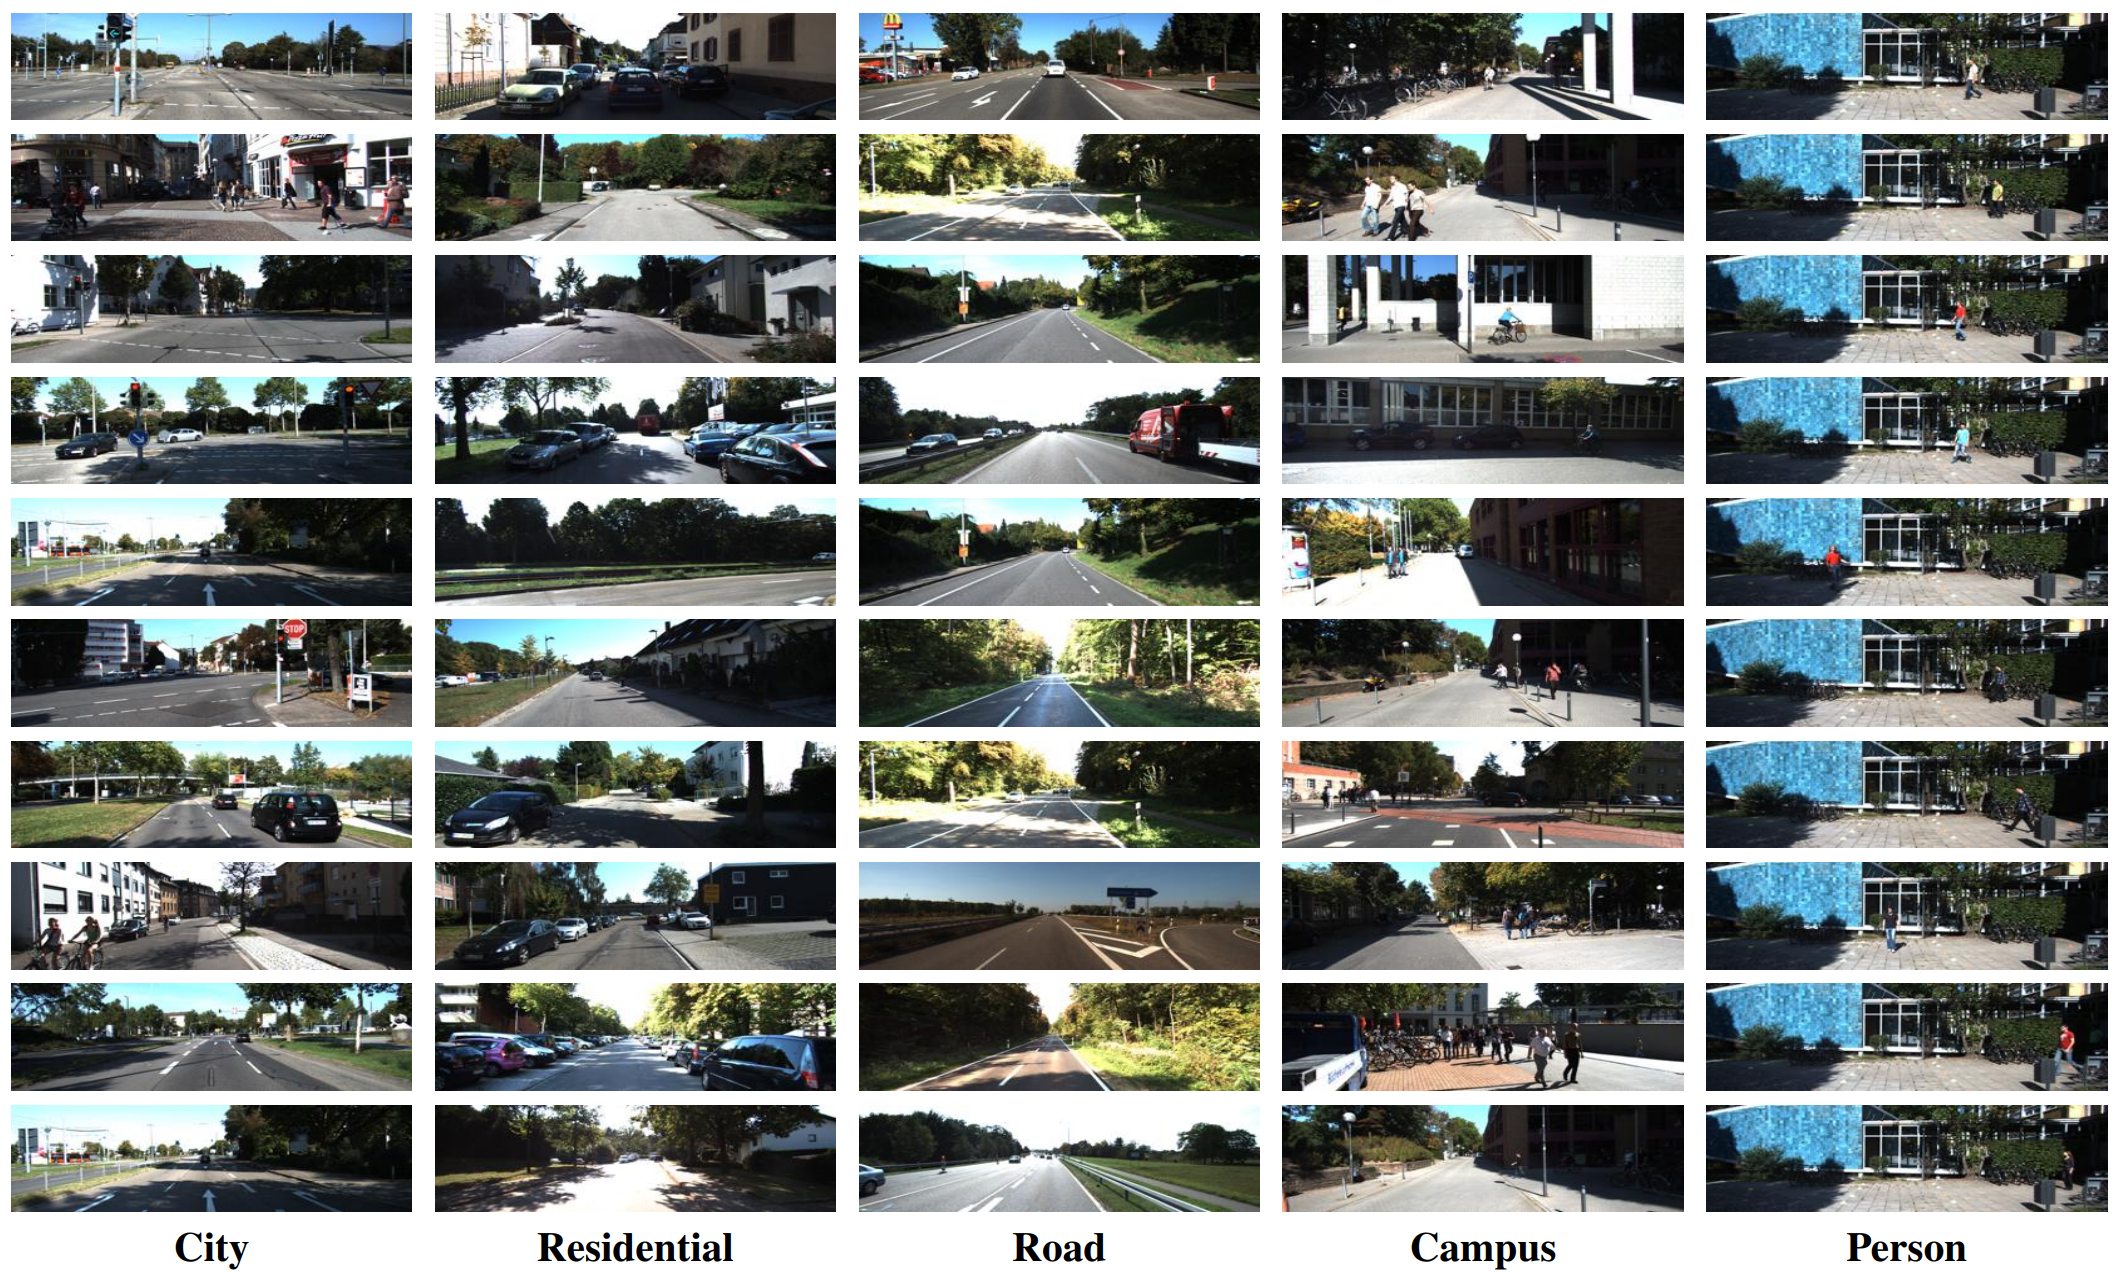
\includegraphics[width=0.9\textwidth]{figures/kitti_exp.png}
	\caption{KITTI数据集示例}
	\label{fig:kitti_exp}
	% \note{注:KITTI数据集丰富多样,包含城市、住宅、道路、校园等不同场景。}
\end{figure}

\begin{figure}[htb]
	\centering
	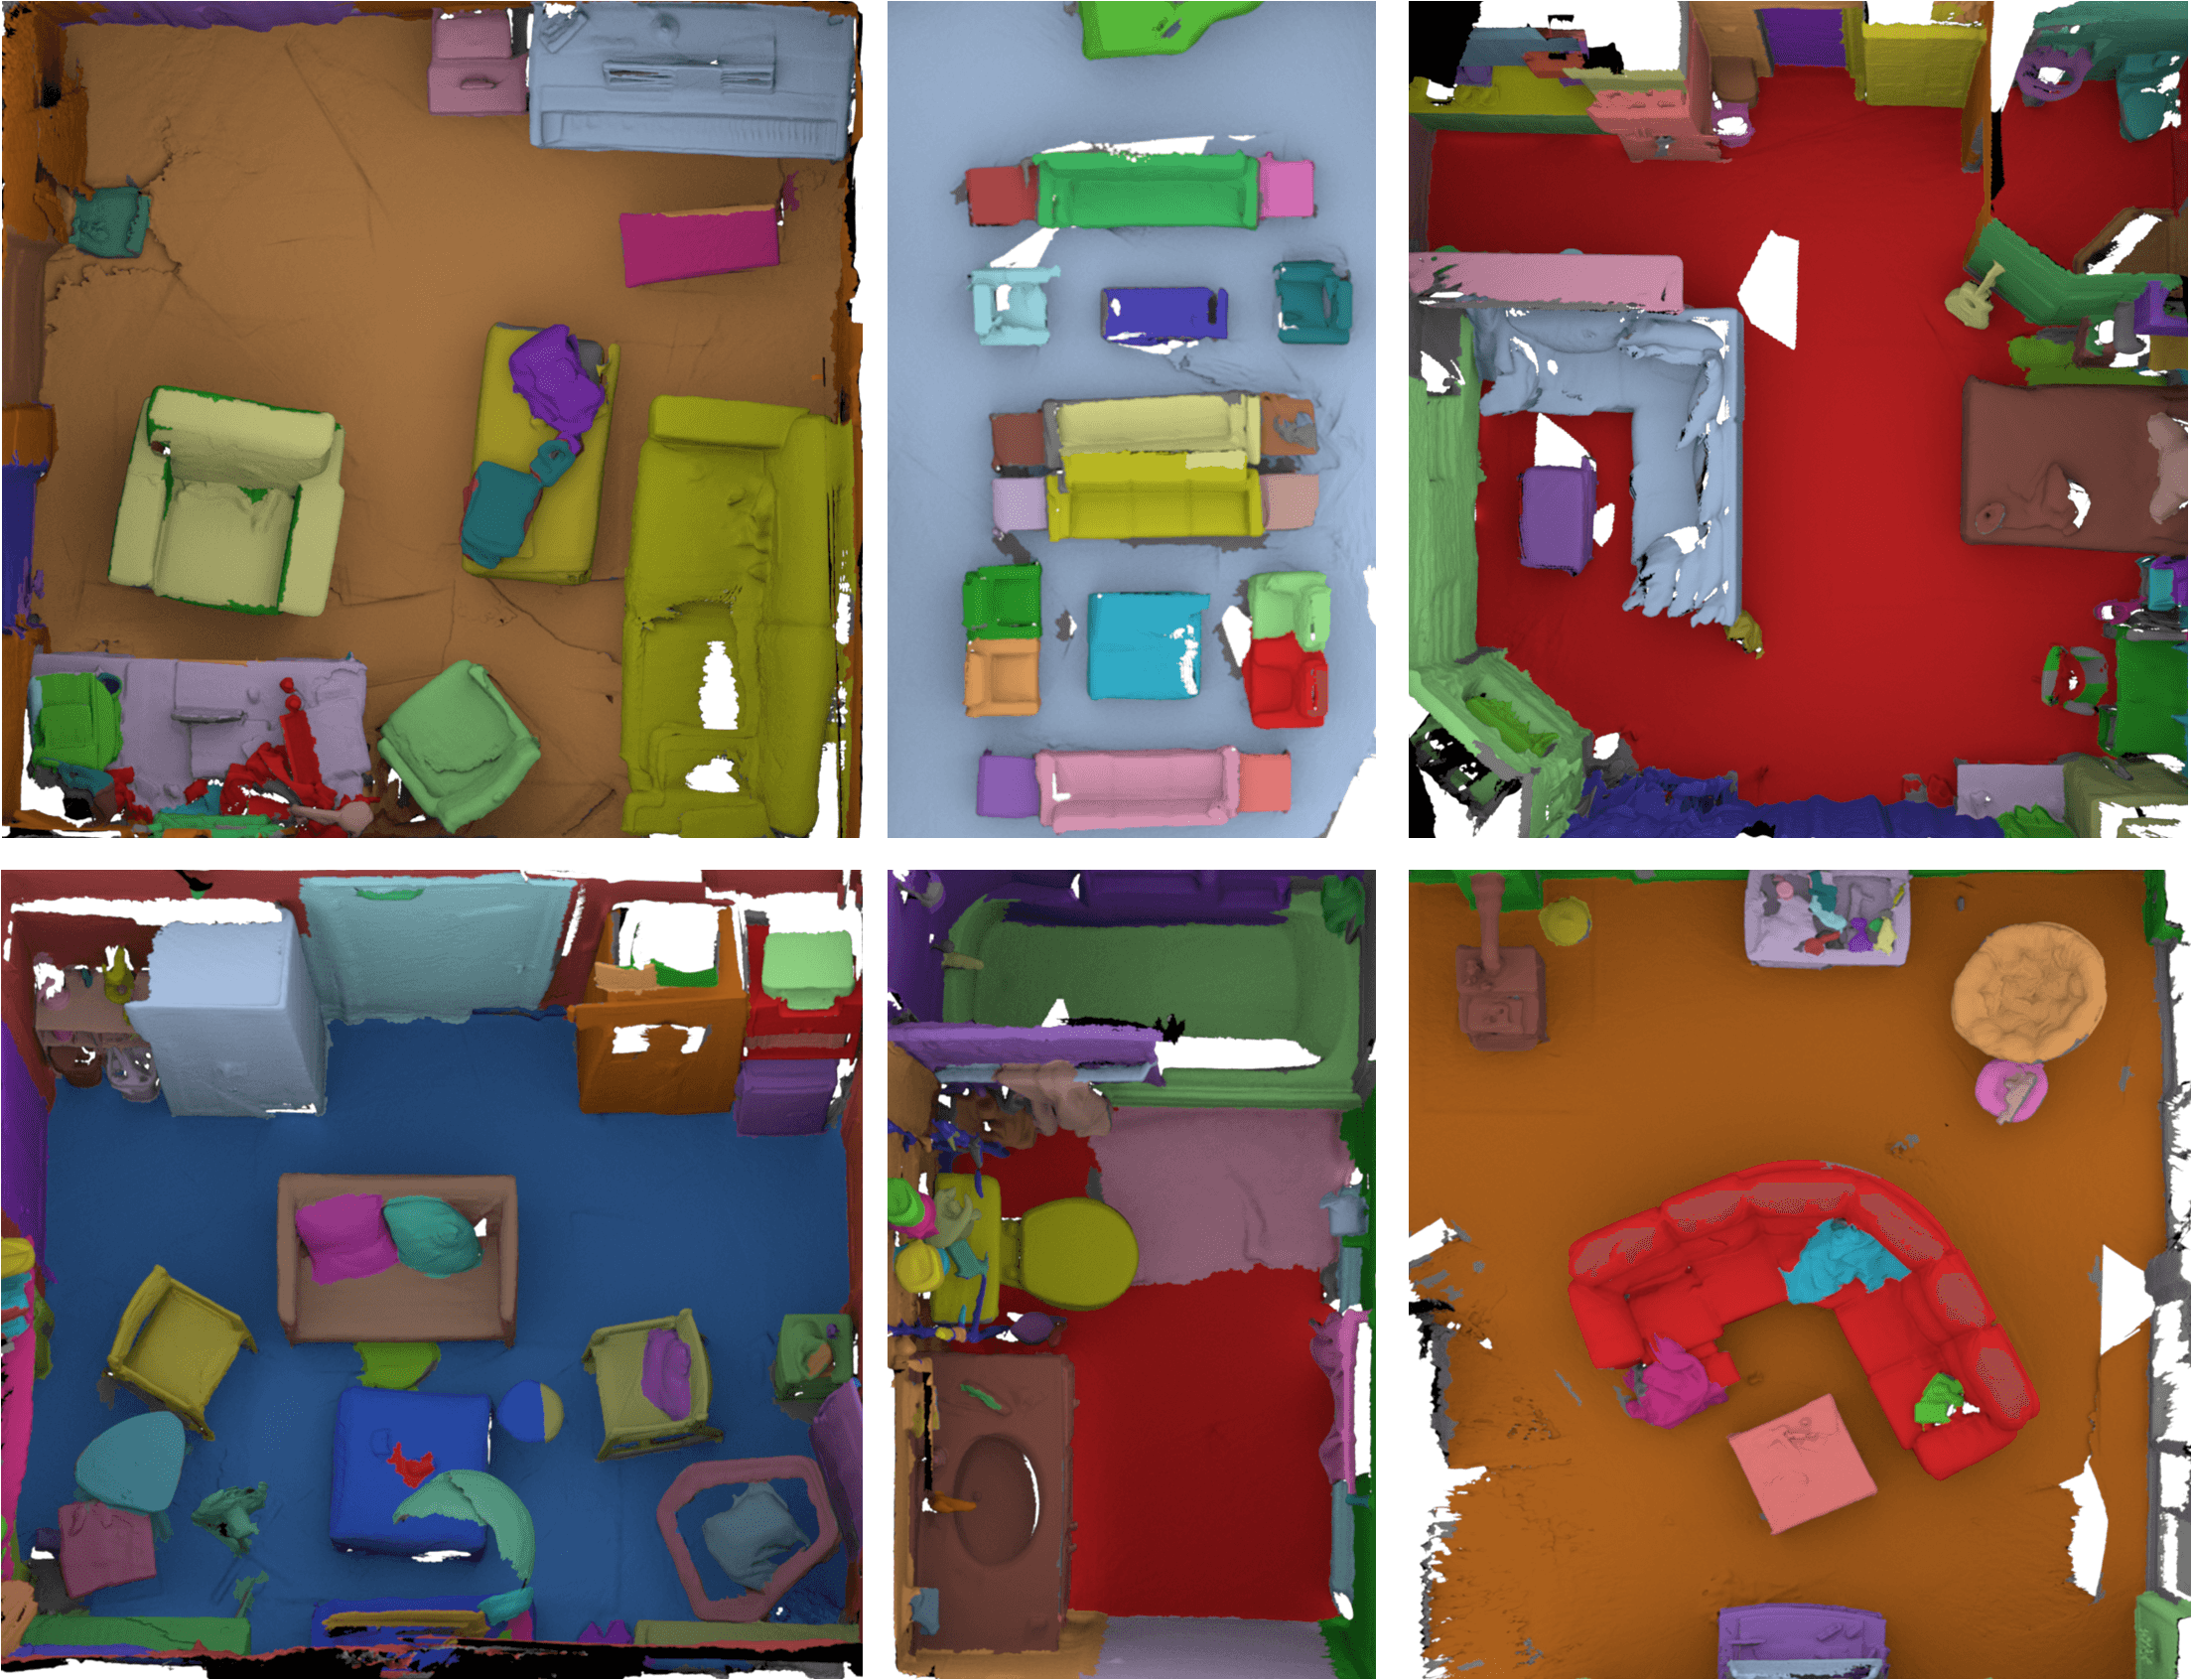
\includegraphics[width=0.9\textwidth]{figures/scannet_exp.png}
	\caption{ScanNet数据集示例}
	\label{fig:scannet}
	\note{注:ScanNet设计了一个易于使用且可扩展的 RGB-D 采集系统,包括自动表面重建和众包语义注释,对场景物体进行实例级别的标签重建。}
\end{figure}

\paragraph{Cityscapes}
Cityscapes是一个用于城市场景理解的大规模数据集。它包含来自50个不同城市的5000个高质量像素级注释图像,分为2975张训练图像,500张验证图像和1525张测试图像。
这些图像覆盖了各种天气条件和日间照明情况。Cityscapes的目标是推进自动驾驶,视觉导航等领域的算法的发展。这个数据集的标注包括30个不同类别,如人、汽车、建筑物、路面等,对于像素级语义分割任务非常有价值。
此外,其中的1740张图像还包含了详细的实例级注释,对于实例分割等任务也非常有帮助。

\paragraph{ScanNet}
ScanNet是一个大规模的三维语义理解数据集,由普林斯顿大学的研究人员在2017年创建。
其数据由RGB-D相机采集产生,使用了一种名为BundleFusion\cite{bundlefusion}的高级三维重建系统,该系统能够实时生成高质量的3D模型。
然后,由人工标注者在三维模型上标注物体,创建类别和实例标签。
ScanNet包含了超过1500个不同的室内场景,涵盖了常见的室内环境,如家庭、办公室、教室等,每个场景都有详细的语义标注,包括物体的类别和每个物体的3D边界框。
如图\ref{fig:scannet}\cite{scannet}所示,数据集中包含了超过20个主要的物体类别,如桌子、椅子、电视等。
此外,ScanNet还提供了一系列基准测试,以评估不同的3D计算机视觉任务,例如语义分割、物体识别和场景分类,并且提供了一个公平的平台,供研究者相互交流。